\documentclass[aspectratio=169]{beamer}

\usepackage[T1]{fontenc}
\usepackage[utf8]{inputenc}
\usepackage{lmodern}
\usepackage{amsmath}
\usepackage{amssymb}
\usepackage{booktabs}
\usepackage{array}
\usepackage{tabularx}
\usepackage{graphicx}
\usepackage{tikz}

\definecolor{CorpBlue}{HTML}{0F4C81}
\definecolor{CorpTeal}{HTML}{1C7C7D}
\definecolor{CorpOrange}{HTML}{D17A22}
\definecolor{CorpLight}{HTML}{F3F6FA}
\definecolor{CorpGray}{HTML}{5B6573}

\usetheme{Madrid}
\setbeamercolor{structure}{fg=CorpBlue}
\setbeamercolor{palette primary}{bg=CorpBlue,fg=white}
\setbeamercolor{palette secondary}{bg=CorpTeal,fg=white}
\setbeamercolor{palette tertiary}{bg=CorpGray,fg=white}
\setbeamercolor{frametitle}{bg=CorpLight,fg=CorpBlue}
\setbeamercolor{block title}{bg=CorpBlue,fg=white}
\setbeamercolor{block body}{bg=CorpLight,fg=black}
\setbeamertemplate{navigation symbols}{}

\newcommand{\code}[1]{\texttt{\small #1}}

\title{NILM -- Nuovi Approcci\\FHMM Survey, HSMM, HiGHS L1-MILP}
\author{}
\date{}

\begin{document}

\begin{frame}
  \titlepage
\end{frame}

% ============================================================
% PANORAMICA
% ============================================================
\begin{frame}{Approcci a Confronto}
  \begin{block}{Obiettivo}
    Confrontare quattro approcci non supervisionati su 6 abitazioni,
    senza ground truth, misurando la qualit\`a di \textbf{ricostruzione del segnale aggregato}.
  \end{block}

  \vspace{0.6em}
  \begin{table}
    \small
    \renewcommand{\arraystretch}{1.2}
    \begin{tabularx}{\textwidth}{l l X}
      \toprule
      \textbf{Approccio} & \textbf{Famiglia} & \textbf{Caratteristica principale} \\
      \midrule
      \code{fhmm\_1\_survey} & FHMM & Baseline always-on + soglia survey-aware \\
      \code{hsmm\_survey}    & HSMM & Viterbi con durata ON esplicita (Gaussiana troncata) \\
      \code{cvxpy\_activation} & L1-MILP (HiGHS) & 3 livelli, penalizzazione accensioni, baseline sottratta \\
      \code{cvxpy\_full}       & L1-MILP (HiGHS) & Always-on come variabili solver, segnale grezzo \\
      \bottomrule
    \end{tabularx}
  \end{table}

  \vspace{0.4em}
  \small
  Granularit\`a: \textbf{15 min} (96 slot/giorno). Segnale troncato a 5 giorni.\\
  Solver MILP: \textbf{HiGHS} (open-source, L1 objective) -- nessuna licenza richiesta.
\end{frame}


% ============================================================
% FHMM_1_SURVEY
% ============================================================
\begin{frame}{FHMM\_1\_Survey -- Idea}
  \small
  \begin{block}{Estensione del FHMM classico}
    Il FHMM modella ogni device come catena di Markov binaria indipendente.
    \code{fhmm\_1\_survey} aggiunge tre livelli di conoscenza di dominio:
  \end{block}

  \vspace{0.4em}
  \begin{enumerate}
    \item \textbf{Baseline always-on:} frigorifero/congelatore stimati upfront e sottratti.
          Il FHMM lavora solo sul residuo $r_t = \max(0,\, y_t - B_{ao})$.
    \item \textbf{Soglia survey-aware:} la soglia di attivazione $\theta_i$ viene moltiplicata
          per fattori derivati dal questionario (finestra oraria, mese attivo).
    \item \textbf{Post-processing:} blocchi ON troppo brevi vengono rimossi;
          potenza stimata dalla pool dei valori del segnale nel blocco.
  \end{enumerate}
\end{frame}

\begin{frame}{FHMM\_1\_Survey -- Formulazione}
  \small
  \textbf{Regola di update coordinato} per device $i$ al tempo $t$:
  \[
    r^{(-i)}_t = y_t - B_{ao} - \sum_{j \neq i} \hat{p}_j\, x_{j,t}
  \]
  \[
    x_{i,t} = \mathbf{1}\!\left[\, r^{(-i)}_t > \theta_i \,\right],
    \qquad
    \theta_i = \frac{p_i}{2} \cdot \varphi_{\text{window}}(i,t) \cdot \varphi_{\text{season}}(i,t)
  \]

  \vspace{0.3em}
  \textbf{Fattori di modulazione dalla survey:}
  \[
    \varphi_{\text{window}}(i,t) =
    \begin{cases}
      0.85 & t \in W_i \text{ (finestra dichiarata)} \\
      1.35 & t \notin W_i
    \end{cases}
    \qquad
    \varphi_{\text{season}}(i,t) =
    \begin{cases}
      0.85 & \text{mese attivo} \\
      1.75 & \text{mese inattivo}
    \end{cases}
  \]

  \vspace{0.3em}
  \textbf{Post-processing:}
  \begin{itemize}
    \item Blocchi ON con durata $< dur\_min\_min_i$ vengono rimossi ($x_{i,t} \leftarrow 0$).
    \item Potenza assegnata: mediana dei valori del residuo nel blocco (non $p_i$ fisso).
  \end{itemize}
\end{frame}

\begin{frame}{FHMM\_1\_Survey -- Risultati}
  \begin{columns}[T]
    \column{0.48\textwidth}
    \centering
    
\includegraphics[width=\textwidth]{images/fhmm_1_survey/86684007269866/2025-11-15.png}
    \footnotesize H1 (86684007269866) -- 2025-11-15

    \vspace{0.5em}
    
\includegraphics[width=\textwidth]{images/fhmm_1_survey/86684007269866/2025-11-20.png}
    \footnotesize H1 (86684007269866) -- 2025-11-20

    \column{0.48\textwidth}
    \centering
    
\includegraphics[width=\textwidth]{images/fhmm_1_survey/86853106211162/2025-11-15.png}
    \footnotesize H4 (86853106211162) -- 2025-11-15

    \vspace{0.5em}
    
\includegraphics[width=\textwidth]{images/fhmm_1_survey/86853106211162/2025-11-20.png}
    \footnotesize H4 (86853106211162) -- 2025-11-20
  \end{columns}
\end{frame}


% ============================================================
% CVXPY_ACTIVATION (prima di hsmm per ordine di complessità)
% ============================================================
\begin{frame}{cvxpy\_activation -- Idea}
  \small
  \begin{block}{L1-MILP con HiGHS (mirror di gurobi\_activation)}
    Stesso modello vincolato di \code{gurobi\_activation} (3 livelli, penalizzazione accensioni,
    finestra soft), ma con \textbf{obiettivo L1} invece di L2 e \textbf{solver HiGHS} (open-source).
  \end{block}

  \vspace{0.4em}
  \textbf{Pipeline:}
  \begin{enumerate}
    \item Baseline always-on stimata e sottratta $\rightarrow$ residuo $s_t$.
    \item Residuo ricampionato a 15 min $\rightarrow$ 96 slot/giorno.
    \item HiGHS risolve il MILP giorno per giorno (\code{time\_limit=60s/giorno}).
    \item Risultato forward-filled a 1 min per benchmark.
  \end{enumerate}

  \vspace{0.3em}
  \textbf{Differenza HiGHS vs Gurobi:}
  \begin{itemize}
    \item Gurobi: $\min \sum_t (s_t - \hat{s}_t)^2$ \quad (L2, quadratica)
    \item HiGHS: $\min \sum_t |s_t - \hat{s}_t|$ \quad (L1, convessa -- riscritta come LP via $e^+_t + e^-_t$)
  \end{itemize}
\end{frame}

\begin{frame}{cvxpy\_activation -- Formulazione MILP}
  \small
  \textbf{Variabili:} $z_{i,t,k}\in\{0,1\}$, $x_{i,t}=\sum_k z_{i,t,k}$,
  $u_{i,t}$ (accensione), $e^+_t, e^-_t \geq 0$ (errore L1).

  \vspace{0.3em}
  \textbf{Livelli di potenza:} $p_{i,0}=(1{-}\eta)p_i,\; p_{i,1}=p_i,\; p_{i,2}=(1{+}\eta)p_i$,\; $\eta=0.15$

  \vspace{0.3em}
  \textbf{Obiettivo:}
  \[
    \min \;\sum_t (e^+_t + e^-_t)
    + \lambda_{tw} \sum_i p_i \sum_{t \notin W_i} x_{i,t}
    + \lambda_{act} \sum_i p_i \sum_t u_{i,t}
  \]

  \textbf{Vincoli principali:}
  \begin{align*}
    &\sum_i \sum_k p_{i,k}\, z_{i,t,k} + e^-_t - e^+_t = s_t \quad\forall t
    \quad\text{(ricostruzione L1)}\\
    &\sum_k z_{i,t,k} \leq 1,\quad x_{i,t} - x_{i,t-1} = u_{i,t} - d_{i,t}
    \quad\text{(transizioni)}\\
    &\sum_{\tau=t}^{t+a_i-1} x_{i,\tau} \geq a_i u_{i,t}
    \quad\text{(durata minima ON)}\\
    &\sum_{\tau=t}^{t+b_i} x_{i,\tau} \leq b_i
    \quad\text{(durata massima ON)}
  \end{align*}
\end{frame}

\begin{frame}{cvxpy\_activation -- Risultati}
  \begin{columns}[T]
    \column{0.48\textwidth}
    \centering
    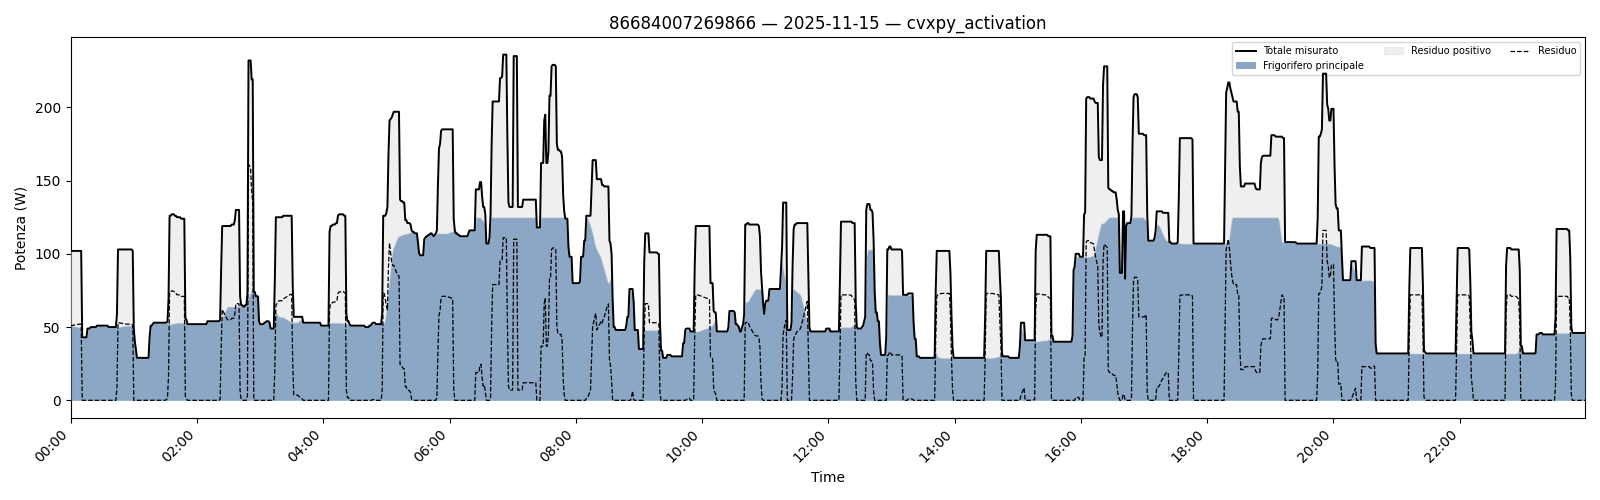
\includegraphics[width=\textwidth]{images/cvxpy_activation/86684007269866/2025-11-15.png}
    \footnotesize H1 (86684007269866) -- 2025-11-15

    \vspace{0.5em}
    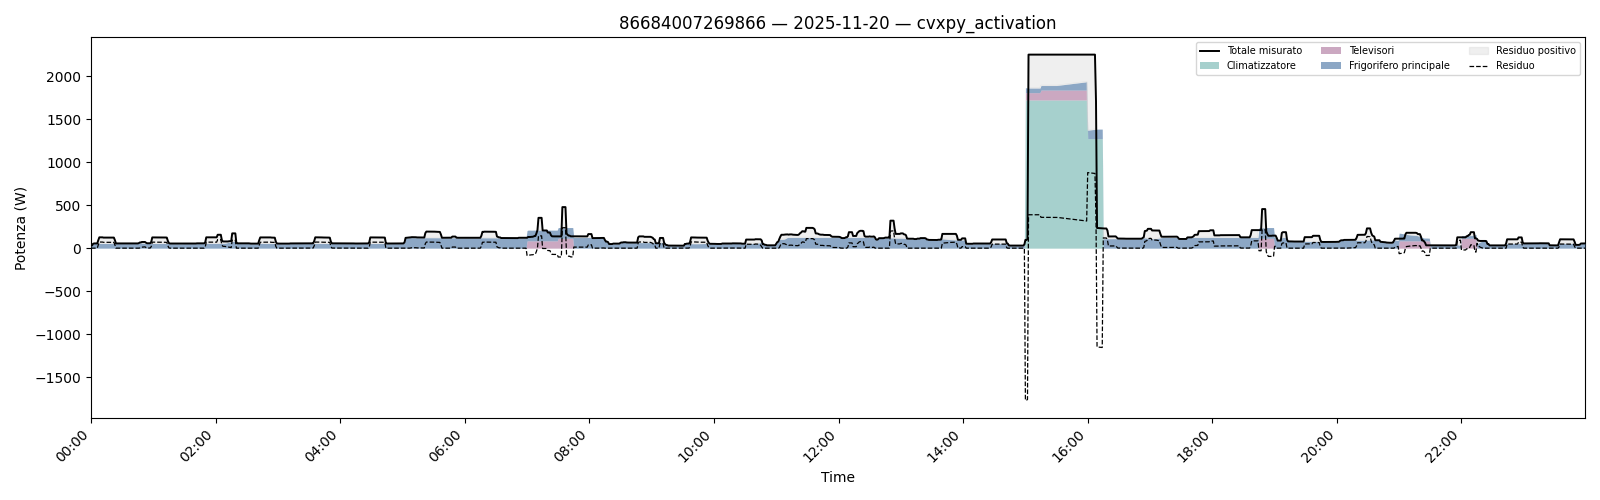
\includegraphics[width=\textwidth]{images/cvxpy_activation/86684007269866/2025-11-20.png}
    \footnotesize H1 (86684007269866) -- 2025-11-20

    \column{0.48\textwidth}
    \centering
    
\includegraphics[width=\textwidth]{images/cvxpy_activation/86853106211162/2025-11-15.png}
    \footnotesize H4 (86853106211162) -- 2025-11-15

    \vspace{0.5em}
    
\includegraphics[width=\textwidth]{images/cvxpy_activation/86853106211162/2025-11-20.png}
    \footnotesize H4 (86853106211162) -- 2025-11-20
  \end{columns}
\end{frame}


% ============================================================
% CVXPY_FULL
% ============================================================
\begin{frame}{cvxpy\_full -- Idea}
  \small
  \begin{block}{Always-on come variabili del solver (mirror di gurobi\_full)}
    Nei modelli precedenti i device \emph{always-on} (frigorifero, congelatore) sono
    stimati upfront e sottratti. In \code{cvxpy\_full} entrano direttamente nel MILP:
    il solver li ottimizza \textbf{congiuntamente} agli event-driven sul \textbf{segnale grezzo}.
  \end{block}

  \vspace{0.4em}
  \textbf{Vantaggio:} elimina l'errore di stima della baseline; il solver trova
  l'assegnazione globalmente ottima di tutti i device.

  \vspace{0.3em}
  \textbf{Suddivisione device:}
  \begin{itemize}
    \item $A$ = always-on (frigorifero, congelatore, \ldots): \emph{sempre attivi},
          esattamente un livello acceso per ogni slot.
    \item $E$ = event-driven (lavatrice, microonde, \ldots): stessi vincoli di
          \code{cvxpy\_activation}.
  \end{itemize}
\end{frame}

\begin{frame}{cvxpy\_full -- Formulazione MILP}
  \small
  \textbf{Variabili always-on:} $z^{ao}_{j,t,k}\in\{0,1\}$,\;
  \textbf{vincolo di uguaglianza:}
  \[
    \sum_{k=0}^{2} z^{ao}_{j,t,k} = 1 \quad \forall j\in A,\,\forall t
    \quad\text{(sempre esattamente un livello attivo)}
  \]

  \textbf{Obiettivo -- segnale grezzo $y_t$, nessuna sottrazione:}
  \[
    \min \;\sum_t (e^+_t + e^-_t)
    + \lambda_{tw} \!\!\sum_{i\in E}\!\! p_i \!\!\sum_{t\notin W_i}\!\! x_{i,t}
    + \lambda_{act} \!\!\sum_{i\in E}\!\! p_i \sum_t u_{i,t}
  \]

  \textbf{Ricostruzione L1:}
  \[
    \sum_{j\in A}\sum_k p_{j,k} z^{ao}_{j,t,k}
    + \sum_{i\in E}\sum_k p_{i,k} z^{ev}_{i,t,k}
    + e^-_t - e^+_t = y_t \quad\forall t
  \]

  Vincoli di transizione, durata minima/massima ON:
  applicati \textbf{solo} ai device event-driven ($E$), identici a \code{cvxpy\_activation}.
\end{frame}

\begin{frame}{cvxpy\_full -- Risultati}
  \begin{columns}[T]
    \column{0.48\textwidth}
    \centering
    
\includegraphics[width=\textwidth]{images/cvxpy_full/86684007269866/2025-11-15.png}
    \footnotesize H1 (86684007269866) -- 2025-11-15

    \vspace{0.5em}
    
\includegraphics[width=\textwidth]{images/cvxpy_full/86684007269866/2025-11-20.png}
    \footnotesize H1 (86684007269866) -- 2025-11-20

    \column{0.48\textwidth}
    \centering
    
\includegraphics[width=\textwidth]{images/cvxpy_full/86853106211162/2025-11-15.png}
    \footnotesize H4 (86853106211162) -- 2025-11-15

    \vspace{0.5em}
    
\includegraphics[width=\textwidth]{images/cvxpy_full/86853106211162/2025-11-20.png}
    \footnotesize H4 (86853106211162) -- 2025-11-20
  \end{columns}
\end{frame}


% ============================================================
% HSMM_SURVEY
% ============================================================
\begin{frame}{hsmm\_survey -- Idea}
  \small
  \begin{block}{Hidden Semi-Markov Model con durata esplicita}
    Estende l'HMM classico permettendo di modellare esplicitamente la
    \textbf{distribuzione della durata} degli stati ON e OFF per ogni device.
    Questo elimina il bias geometrico dell'HMM (che favorisce cicli molto brevi o molto lunghi).
  \end{block}

  \vspace{0.4em}
  \textbf{Distribuzioni di durata (parametri dalla survey):}
  \begin{itemize}
    \item \textbf{ON:} Gaussiana troncata con media $\mu = dur\_typical\_min / \Delta t$
          e $\sigma = \mu / 3$, troncata in $[dur\_min, dur\_max]$.
    \item \textbf{OFF:} Geometrica con parametro $q$ calibrato sulla frequenza settimanale dichiarata.
  \end{itemize}

  \vspace{0.3em}
  \textbf{Emissione:} Gaussiana su potenza con bias logaritmico survey-aware
  (finestra oraria, mese attivo).
\end{frame}

\begin{frame}{hsmm\_survey -- Formulazione Viterbi}
  \small
  \textbf{DP per device $i$, giorno con $T$ slot:}

  \vspace{0.3em}
  \textbf{Stato ON, durata residua $d$:}
  \[
    V^{on}_{i}(t, d) = \max_{d' \geq d}
    \left[
      V^{on}_{i}(t{-}1, d{+}1) + \log \mathcal{N}(r^{(-i)}_t;\, p_i, \sigma^2_i)
      + \text{bias}_{survey}(i,t)
    \right]
  \]

  \textbf{Stato OFF:}
  \[
    V^{off}_{i}(t) = \max \left[
      V^{off}_{i}(t{-}1) + \log q_i,\quad
      \max_{d} V^{on}_{i}(t{-}1, d) \cdot \mathbf{1}[d = d_{min}]
    \right]
  \]

  \textbf{Transizione OFF$\to$ON} con distribuzione durata $P_{dur}(d)$:
  \[
    V^{on}_{i}(t, d_{max}) = V^{off}_{i}(t{-}1) + \log P_{dur}(d_{max})
  \]

  \vspace{0.3em}
  \small
  La complessit\`a \`e $O(T \cdot d_{max})$ per device per iterazione.
  Ottimizzazione: prefix-sum per sommare emissioni in blocchi ON contigui.
\end{frame}

\begin{frame}{hsmm\_survey -- Risultati}
  \begin{columns}[T]
    \column{0.48\textwidth}
    \centering
    
\includegraphics[width=\textwidth]{images/hsmm_survey/86684007269866/2025-11-15.png}
    \footnotesize H1 (86684007269866) -- 2025-11-15

    \vspace{0.5em}
    
\includegraphics[width=\textwidth]{images/hsmm_survey/86684007269866/2025-11-20.png}
    \footnotesize H1 (86684007269866) -- 2025-11-20

    \column{0.48\textwidth}
    \centering
    
\includegraphics[width=\textwidth]{images/hsmm_survey/86853106211162/2025-11-15.png}
    \footnotesize H4 (86853106211162) -- 2025-11-15

    \vspace{0.5em}
    
\includegraphics[width=\textwidth]{images/hsmm_survey/86853106211162/2025-11-20.png}
    \footnotesize H4 (86853106211162) -- 2025-11-20
  \end{columns}
\end{frame}


% ============================================================
% CONFRONTO SOLVER
% ============================================================
\begin{frame}{Solver: HiGHS vs Gurobi}
  \small
  \begin{table}
    \renewcommand{\arraystretch}{1.3}
    \begin{tabularx}{\textwidth}{l X X}
      \toprule
      & \textbf{HiGHS} & \textbf{Gurobi} \\
      \midrule
      Licenza & Open-source (MIT) & Commerciale (accademica gratis) \\
      Tipo & LP + MILP puro & LP + MILP + MIQP \\
      Obiettivo & \textbf{L1} (convessa, riscritta come LP) & \textbf{L2} (quadratica) \\
      Penalizzazioni & $\lambda \cdot p_i$ & $\lambda \cdot p_i^2$ \\
      Velocit\`a MILP & Molto buona & Migliore su problemi grandi \\
      Uso in questo progetto & \code{cvxpy\_activation}, \code{cvxpy\_full} & \code{gurobi\_activation}, \code{gurobi\_full} \\
      \bottomrule
    \end{tabularx}
  \end{table}

  \vspace{0.5em}
  \small
  \textbf{Nota:} le penalizzazioni scalano diversamente perch\'e con L1 l'unit\`a
  dell'obiettivo \`e $[\mathrm{W}]$ mentre con L2 \`e $[\mathrm{W}^2]$.
  Il termine $\lambda_{act} \cdot p_i$ in HiGHS equivale al costo di uno slot di ricostruzione nulla.
\end{frame}


% ============================================================
% METRICA E BENCHMARK
% ============================================================
\begin{frame}{Metrica: MAE di Ricostruzione}
  \small
  In assenza di ground truth, la metrica usata misura quanto bene la somma
  delle disaggregazioni ricostruisce il segnale aggregato:

  \[
    \mathrm{MAE}_{\mathrm{recon}} = \frac{1}{T}\sum_{t=1}^{T}
    \left|\, y_t - \sum_i \hat{w}_i(t) \,\right|
  \]

  \begin{block}{Nota}
    Un MAE basso indica buona ricostruzione, \textbf{non} necessariamente
    corretta attribuzione per device -- la disaggregazione potrebbe essere
    corretta anche con assegnazioni sbagliate.
  \end{block}

  \vspace{0.4em}
  \textbf{Approcci a confronto su tutti gli IMEI disponibili:}
  \begin{itemize}
    \item \code{fhmm\_1\_survey}: veloce, survey-aware, nessun solver esterno.
    \item \code{cvxpy\_activation}: MILP L1, baseline sottratta, $\sim$60s/giorno.
    \item \code{cvxpy\_full}: MILP L1, always-on nel solver, $\sim$60s/giorno.
    \item \code{hsmm\_survey}: DP semi-Markoviana, durata esplicita, $\sim$iterativo.
  \end{itemize}
\end{frame}

\end{document}
